\section{Window Layout Concept}
    Developers can define their working environment to fit the needs and preferences. For a better understanding of
    further comments and instructions, lets define five major areas of the main window.

   \begin{figure}[h]
        \centering
        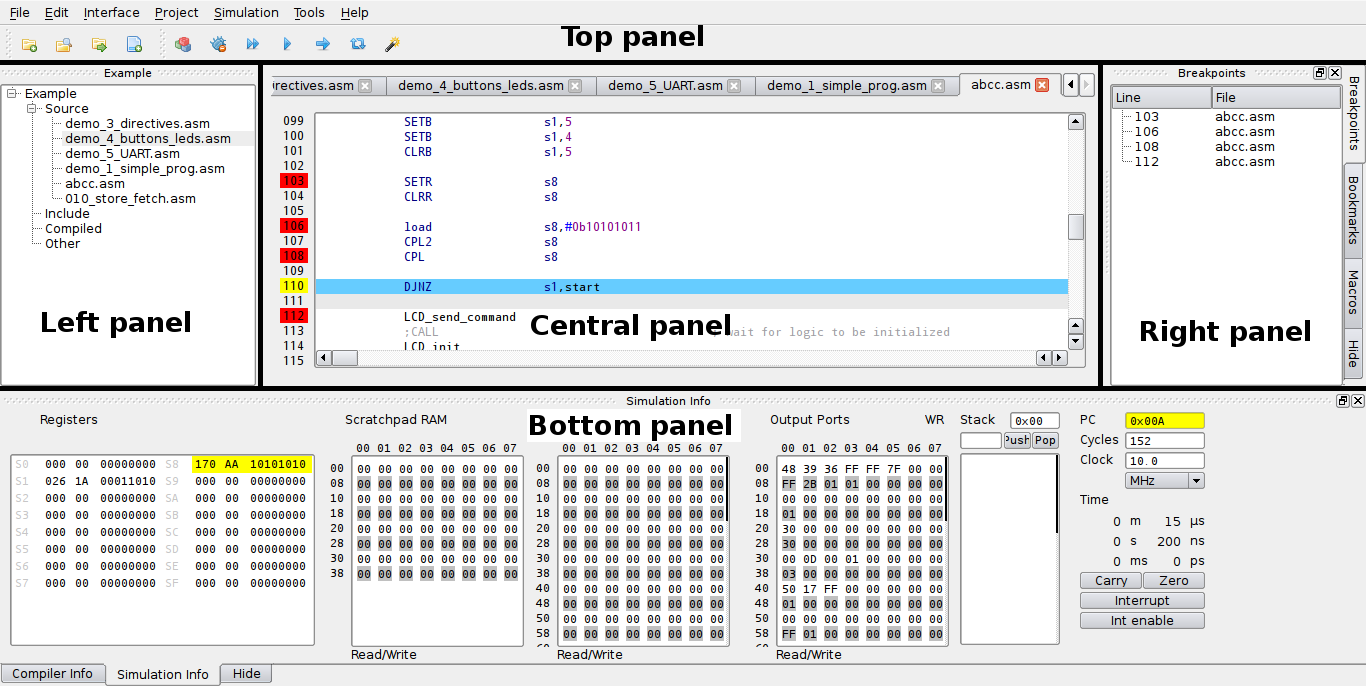
\includegraphics[width=\textwidth]{img/Main_window.png}
        \caption{Window layout concept}
    \end{figure}

\subsection{Central panel}
    Central panel contains the main text editor with syntax highlight for writing a source code. In the editor you can
    also easily add breakpoints and bookmarks just by clicking on desired line number by left or right mouse button,
    each invokes different action.

\subsection{Top panel}
   \begin{figure}[h!]
        \centering
        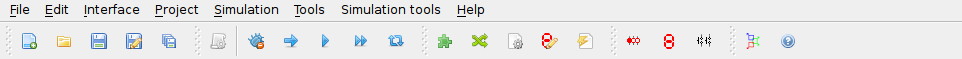
\includegraphics[width=0.75\textwidth]{img/top_panel.png}
        \caption{Toolbar icons}
    \end{figure}

\subsubsection{Top panel icons}
    \begin{itemize}
        \item New project: Creates a new project.
        \item Open project: Opens an existing project file.
        \item Save project: Saves current project file.
        \item Compile: Compiles your code.
        \item Start Simulation: Enters simulation mode.
        \item Run: High speed simulation.
        \item Animate: Simulation with GUI (such as register view, etc.) updated after each executed instruction.
        \item Step: Step by step simulation.
        \item Reset: Resets simulator to its initial state.
        \item Unhighlight: Clear highlight from register view and other graphical components of the simulator panel.
        \item Undo: will undo all edit actions on the open document in reverse order
        \item Redo: will redo all undo actions
        \item Cut: cuts all selected parts of the open document and puts it in the clipboard.
        \item Copy: copies all selected parts of the open document to the clipboard
        \item Paste: pastes the text contents of the clipboard in the open document
        \item Select: All selects all text in the open document
        \item Find: find a to be given string through the open document
        \item Replace: replace a given string in the open document by a new string
    \end{itemize}

\subsection{Bottom panel}
    Bottom panel consists of simulator main panel, and compiler messages.

    In simulator main panel you can see status of internal registers, scratch-pad ram, input and output ports, call
    stack, program counter, elapsed time and machine cycles, processor clock, and internal flags carry and zero. All
    these values can be edited during processor simulation.

    In compiler messages panel you can see textual output from the assembler, like warnings and other messages.

    \begin{figure}[h!]
        \centering
        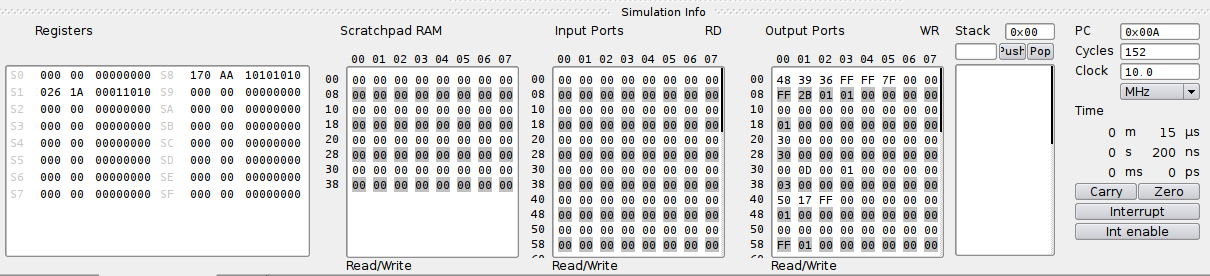
\includegraphics[width=\textwidth]{img/bottom_panel.png}
        \caption{Bottom panel}
    \end{figure}

\subsection{Left panel}
    Here you can see main project tree. You can close or configure project by right clicking on the project name, add a
    file to the project or create a new one. You can also see included files or opened compiled files like .lst, etc.

\subsection{Right panel}
    Right panel contains lists of breakpoints, bookmarks, symbols, and macros in your source code.

    \begin{table}[h!]
        \begin{tabular}{cc}
            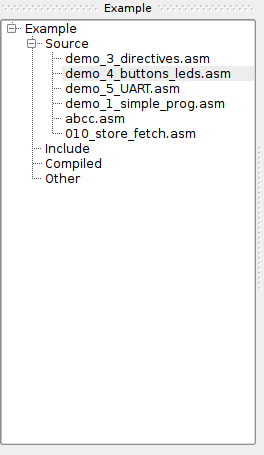
\includegraphics[width=.33\textwidth]{img/left_panel.png}
                &
            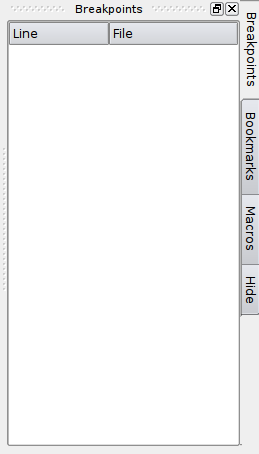
\includegraphics[width=.33\textwidth]{img/right_panel.png}
                \\
            Left panel & Right panel
        \end{tabular}
    \end{table}

\clearpage

\subsection{Project configuration}
    In project configuration window, you can edit project and compiler settings. You can open project configuration
    window by right clicking on project name in the left panel and choosing Configuration, see the pictures below.
    This will open main configuration window with multiple tabs on the left side.

    \subsubsection{Project - Options}
        \begin{itemize}
            \item Project name: Name of your project.
            \item Architecture: Processor architecture for your project.
            \item Family: Processor family of the selected architecture.
            \item Info panel: Brief description of selected processor.
        \end{itemize}

        \subsubsection{Project - Memory}
            \begin{itemize}
                \item Size options: Tell the compiler your processor's memory size.
                \item Interrupt vector: Set your interrupt vector (size of program memory - 1 is maximum),
                \item HW build: Your HW build constant.
            \end{itemize}

        \begin{table}[h!]
            \begin{tabular}{cc}
                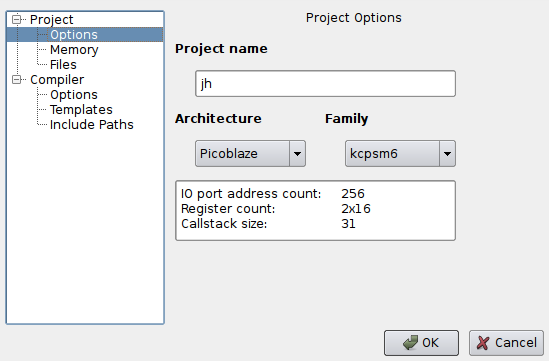
\includegraphics[width=.5\textwidth]{img/config2.png}
                    &
                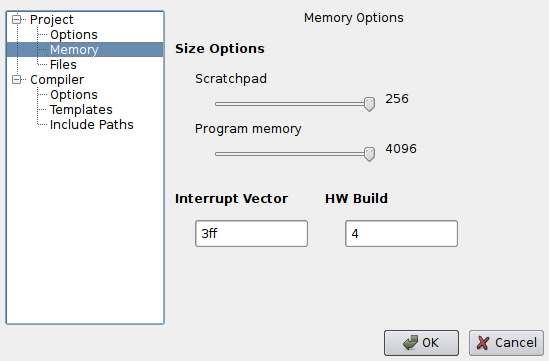
\includegraphics[width=.5\textwidth]{img/config1.png}
                    \\
                Project - Options & Project - Memory
            \end{tabular}
        \end{table}

    \subsubsection{Project - Files}
        Here is where you can create, add, or remove files from your project, and set set the main file (see below).

    \clearpage

    \subsubsection{Compiler - Options}
            \begin{itemize}
                \item Main file: If you have "Use main file" checked, you can choose which file will always chosen for
                      compilation and simulation instead of the file current opened in the editor.
                \item Generate: Select which files should the assembler generate in your project's directory from the
                      given source code.
            \end{itemize}

        \begin{table}[h!]
            \begin{tabular}{cc}
                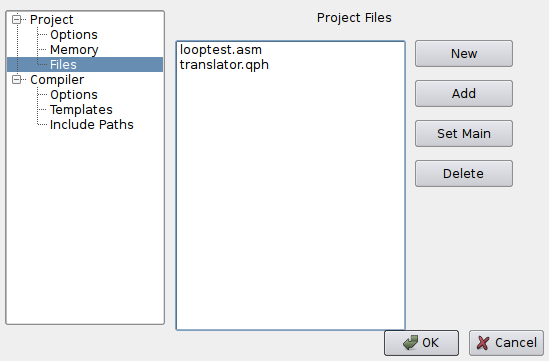
\includegraphics[width=.5\textwidth]{img/config3.png}
                    &
                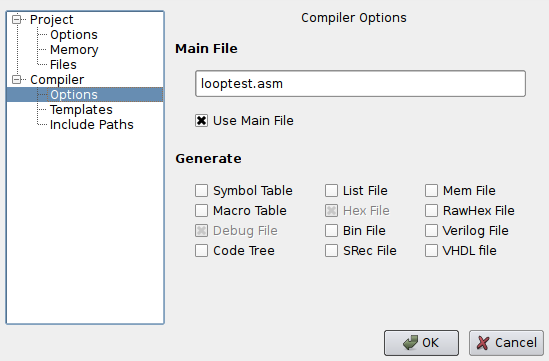
\includegraphics[width=.5\textwidth]{img/config4.png}
                    \\
                Project - Files & Compiler - Options
            \end{tabular}
        \end{table}

        \subsubsection{Compiler - templates}
            Choose which VHDL or Verilog template will be used by the assembler to generate the HDL code for your
            design, by default MDS uses its own built-in templates which.

        \subsubsection{Compiler - include paths}
            Here you can add or edit path, where the compiler will try to find files included in other source code files
            (directive INCLUDE).

        \begin{table}[h!]
            \begin{tabular}{cc}
                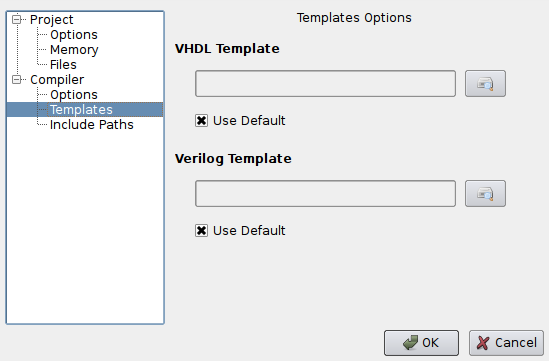
\includegraphics[width=.5\textwidth]{img/config5.png}
                    &
                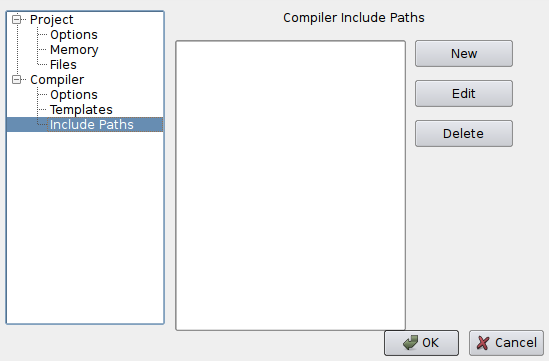
\includegraphics[width=.5\textwidth]{img/config6.png}
                    \\
                Compiler - Templates & Compiler - Include paths
            \end{tabular}
            \end{table}

\subsection{Interface configuration}
    In interface configuration dialog, you can edit IDE behavior and appearance, for instance editor font, tab width,
    etc., or simulator warnings. To open the interface configuration dialog, click on [Main~Menu] -> [Interface] ->
    [Config].

    \subsubsection{IDE - General}
        In the general settings you can set if you want splash screen, session restoration, or change language of whole
        IDE (this option is available only when language pack for your language is available.).

    \subsubsection{Editor - General}
        General settings of IDE editor. You can set tab width, number of spaces .

        \begin{table}[h!]
            \begin{tabular}{cc}
                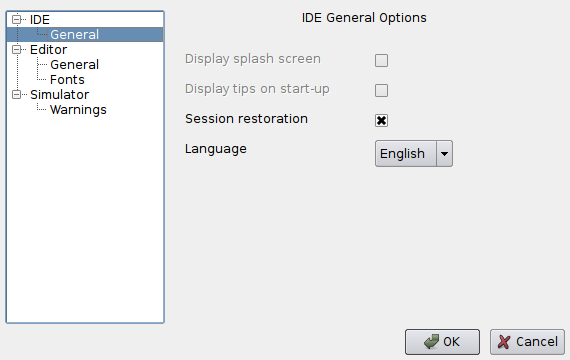
\includegraphics[width=.5\textwidth]{img/interface1.png}
                    &
                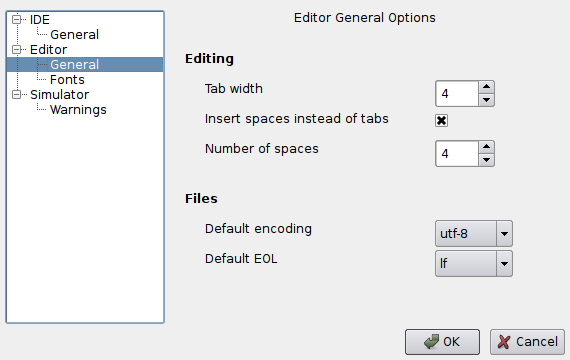
\includegraphics[width=.5\textwidth]{img/interface2.png}
                    \\
                IDE - General & Editor - General
            \end{tabular}
        \end{table}

        \begin{table}[h!]
            \begin{tabular}{cc}
                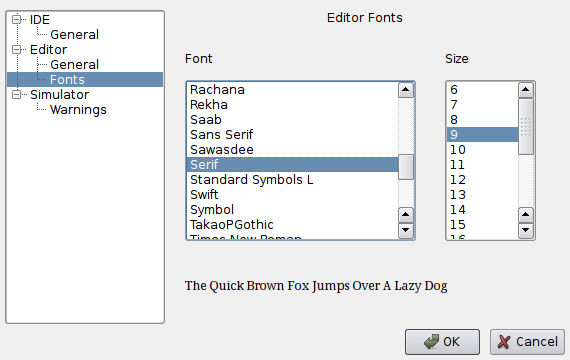
\includegraphics[width=.5\textwidth]{img/interface3.png}
                    &
                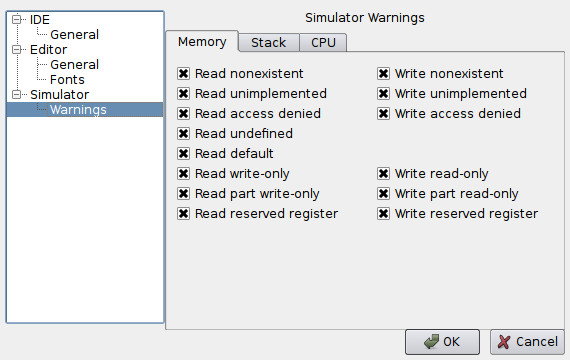
\includegraphics[width=.5\textwidth]{img/interface4.png}
                    \\
                Editor - Fonts & Simulator - Warnings -> Memory
            \end{tabular}
        \end{table}

        \begin{table}[h!]
            \begin{tabular}{cc}
                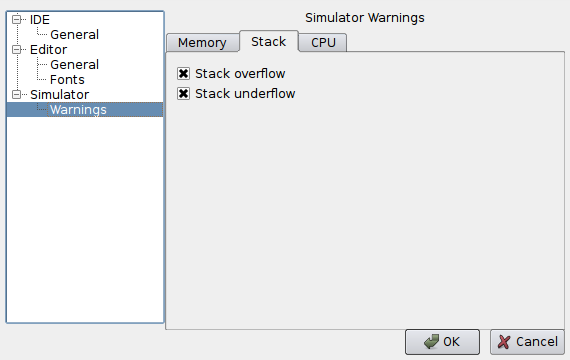
\includegraphics[width=.5\textwidth]{img/interface5.png}
                    &
                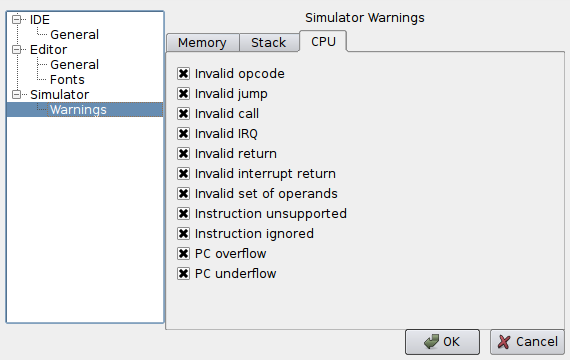
\includegraphics[width=.5\textwidth]{img/interface6.png}
                    \\
                Simulator - Warnings -> Stack & Simulator - Warnings -> CPU
            \end{tabular}
        \end{table}


\subsection{Other tools}

\subsection{DATA file convertor}
    This tool allows you to convert selected data file to another. Mutual conversion can be made between .ihex, .bin,
    .srec, .mem, .rawhex, .v, and .vhd.
    \begin{description}
        \item[Section Input File] Here you can select desired input data file which is going to be converted
        \item[Section Input Options] In this section, you define what type of input file is going to be converted
        \item[Input file type] Available options - Hex, Bin, SRec, XilMem, XilVerilog and XilVhdl
        \item[Bytes per record] Only if you want to convert XilMem file. Defines number of bytes per record
        \item[OPCode size] Defines opcode size of selected data file. Available are 16 and 18
        \item[Section Output File] Defines target
        \item[Section Output Options] Here you can select desired output data file.
        \item[Input file type] Available options - Hex, Bin, SRec, XilMem, XilVerilog and XilVhdl.
        \item[Tab size]  Define number of inserted spaces when you press Tab.
        \item[Short instructions] Here you can allow short instructions like LD, RETI or others
    \end{description}

    \begin{figure}[h]
        \centering{}
        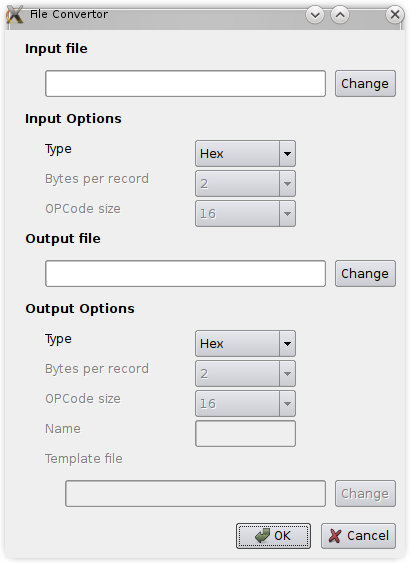
\includegraphics[width=.5\textwidth]{img/DATA_convertor.png}
        \caption{DATA file convertor}
    \end{figure}

\subsection{ASM translator}
    With this tool, you can translate your previously written assembler code in different syntax.
    You can sellect one of three choices - Xilinx, Mediatronix and OpenPicIde. Input code should be without
    errors.
    \begin{description}
        \item[Section Input File] Here you can choose which file you want to translate into the MDS assembler
        \item[Section ASM type] Input file syntax version. Translator needs to know input file syntax. Select one of three choices - Xilinx, Mediatronix and OpenPicIde
        \item[Symbol] Case of symbols - UPPERCASE or LOWERCASE
        \item[End of line] Indentation - Choose between Tabs or Spaces
        \item[Directive] Case of Directives - UPPERCASE or LOWERCASE
        \item[Indentation] Three choices - Tabs, Spaces and Keep (indentation unchanged)
        \item[Instruction] Case of instructions - UPPERCASE or LOWERCASE
        \item[Tab size]  Define number of inserted spaces when you press Tab.
        \item[Short instructions] Here you can allow short instructions like LD, RETI or others
    \end{description}

    \begin{figure}[h]
        \centering{}
        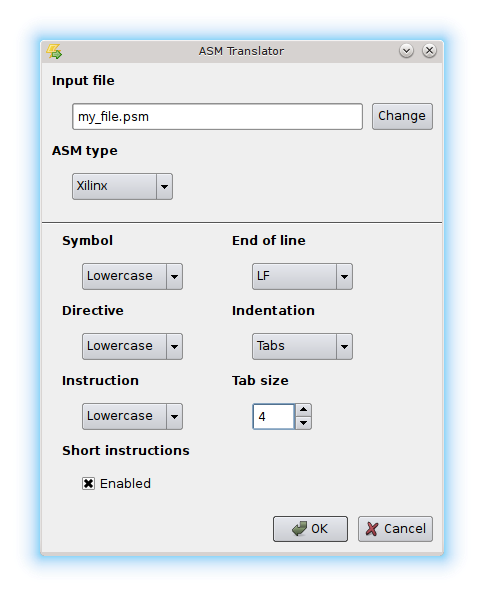
\includegraphics[width=.5\textwidth]{img/ASM_translator.png}
        \caption{ASM translator}
    \end{figure}

\subsection{Disassembler}
    A disassembler is a tool that translates machine language into assembly language. The inverse
    operation to that of an assembler.

    \begin{description}
        \item[Section File] Here you can choose which file you want to be disassembled
        \item[Section Target] Architecture - Select processor architecture
        \item[Family] select processor family of selected architecture
        \item[Section Options] Indentation - Choose between Tabs or Spaces
        \item[TabSize] Number of spaces in one tab
        \item[Radix] Binary,Octal, Decima or Hexadecimal
        \item[Linebreak] LF,CR or CRLF
        \item[Case]  You can choose if you want disassemled file will be in upper or lower case
        \item[Generate symbols] Select which symbols should be disassembled
    \end{description}

    \begin{figure}[h]
        \centering{}
        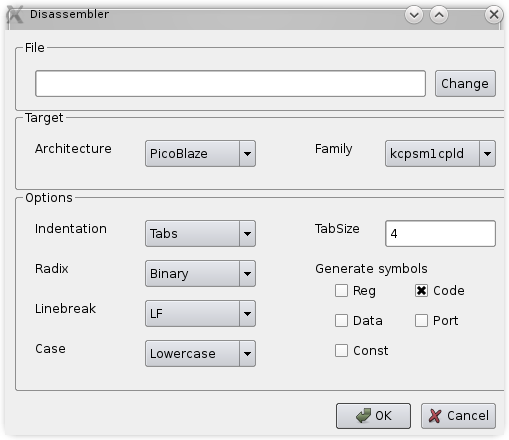
\includegraphics[width=.5\textwidth]{img/disassembler_window.png}
        \caption{Disassembler}
    \end{figure}

\subsection{Waiting loop generator}
    In many cases, it is usefull to have a tool for creating waiting loops. It can save some time in development process. This tool can generate
    waiting loops using up to six registers. All you have to do is insert desired waiting time or number of cycles and valid frequency.

    \begin{description}
        \item[Section Input variable] You can choose between time or cycles
        \item[Section Desired waiting time] Insert number of executed time or cycles
        \item[Section Frekvency] Set working frequency
        \item[Section Register names] Optional selection. You can change register names in generated code
        \item[Section Generated code] Here is where code will appear
        \item[Instruction] Select instruction used in loop.
        \item[Type] Type of waiting loop you want to create (blank/macro).
        \item[Checkboxes UpperCase and Comments]  You can turn off automaticaly added comments or change letter case
        \item[Button Copy to clipboard] This will copy loop into your clipboard
        \item[Button Generate] When you have all set. This will generate loop
    \end{description}

    \begin{figure}[h]
        \centering{}
        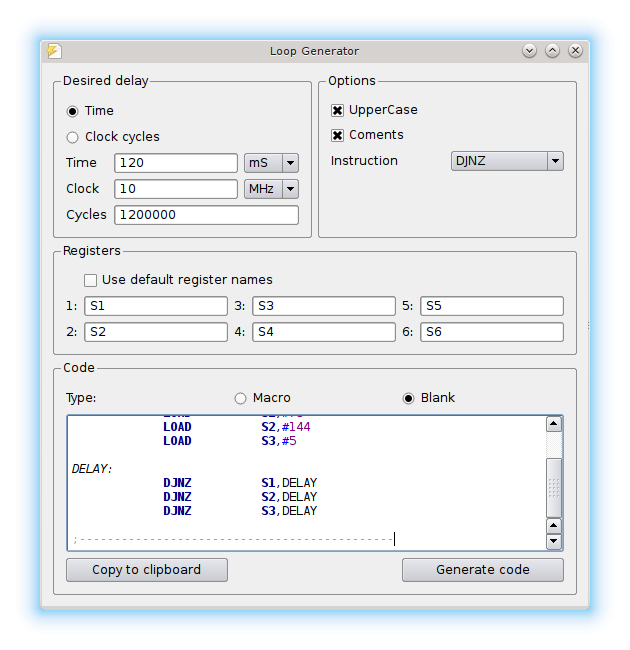
\includegraphics[width=.7\textwidth]{img/loop_gen.png}
        \caption{Loop generator user interface}
    \end{figure}

\subsection{8-segment editor}
    \begin{wrapfigure}{r}{0pt}
        \centering{}
        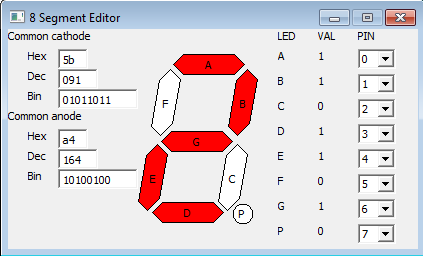
\includegraphics[width=110pt]{img/8segment.png}
        \caption{8-segment editor}
    \end{wrapfigure}
    With this tool you can easily determine what value you have to set on a port to display a digit on a numerical LED display. In the left part of the dialog window, you can find numerical val ues corresponding to the digit displayed in the middle part. These values are represented for both common cathode and anode and in three numerical bases, hexadecimal, decimal and oc tal. Buttons on left side from entry boxes copies value from adjacent entry box into clipboard. In the right part of the window you can set what port pin is connected to what LED segment.

\subsection{LED panel simulator}
    \begin{wrapfigure}{r}{0pt}
        \centering{}
        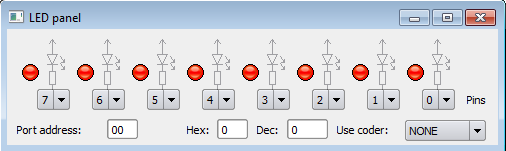
\includegraphics[width=150pt]{img/Led_panel.png}
        \caption{8-segment editor}
    \end{wrapfigure}
    Simple LED panel simulator. You can observe output port behavior with visual presentation of eight leds. You can activate coder to simulate common FPGA logic.

    \begin{description}
        \item[GRAY] Converts output port value to gray code.
        \item[BCD] Output port value will be presented as BCD. Remember that bigger number than 99 cannot be displayed.
    \end{description}

\subsection{7-segment simulator}
    \begin{wrapfigure}{r}{0pt}
        \centering{}
        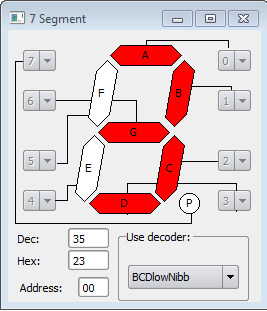
\includegraphics[width=110pt]{img/7seg_sim.png}
        \caption{7-segment simulator}
    \end{wrapfigure}
    Simulator of 7-segment display connected to output port(common anode). PORT bits can be assigned to any display segment. Multiple instances of simulator can be opened at once.
    You can activate decoder to simulate commonly used FPGA logic.
    \begin{description}
        \item[BCDlowNibb] Output port low nibble is displayed.
        \item[BCDhighNibb] Output port high nibble is displayed.
    \end{description}

\subsection{Number base converter}
    \begin{wrapfigure}{r}{0pt}
            \centering
            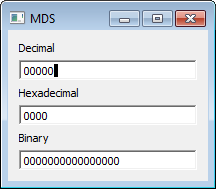
\includegraphics[width=90pt]{img/convertor.png}
            \caption{Convertor}
    \end{wrapfigure}
    This tool is very usefull, when you want to find out the representation of given number in other number bases.
